
%% Electromagnetic Application Questions used
%% on the NYSED Physics Regents Examination
%%--------------------------------------------------

%% this section contains 86 problems


%% Section June2015
%%--------------------
\element{nysed}{
\begin{question}{June2015-Q14}
    Which energy transformation occurs in an
        operating electric motor?
    \begin{choices}
      \correctchoice{electrical$\rightarrow$mechanical}
        \wrongchoice{chemical$\rightarrow$electrical}
        \wrongchoice{mechanical$\rightarrow$electrical}
        \wrongchoice{electrical$\rightarrow$chemical}
    \end{choices}
\end{question}
}


%% NOTE: Jan2002 is the last exam to include Electromagnetic Application


%% Section Jan2002
%%--------------------
\element{nysed}{
\begin{question}{Jan2002-Q76}
    If the current in an ammeter's coil is doubled,
        the resulting torque on the coil will be
    \begin{multicols}{2}
    \begin{choices}
        \wrongchoice{unchanged}
      \correctchoice{doubled}
        \wrongchoice{halved}
        \wrongchoice{quadrupled}
    \end{choices}
    \end{multicols}
\end{question}
}

\element{nysed}{
\begin{question}{Jan2002-Q77}
    An operating electric motor induces an EMF in the armature
        that opposes the applied potential difference.
    This phenomenon is an example of conservation of
    \begin{multicols}{2}
    \begin{choices}
        \wrongchoice{inertia}
        \wrongchoice{electric charge}
        \wrongchoice{momentum}
      \correctchoice{energy}
    \end{choices}
    \end{multicols}
\end{question}
}

\element{nysed}{
\begin{question}{Jan2002-Q78}
    The rate of thermionic emission from a surface increases as the surface's
    \begin{choices}
        \wrongchoice{temperature decreases}
        \wrongchoice{thickness decreases}
      \correctchoice{temperature increases}
        \wrongchoice{thickness increases}
    \end{choices}
\end{question}
}

\element{nysed}{
\begin{question}{Jan2002-Q79}
    An electron moves at \SI{2.0e6}{\meter\per\second}
        perpendicular to a magnetic field having a flux density of \SI{2.0}{\tesla}.
    What is the magnitude of the magnetic force on the electron?
    \begin{multicols}{2}
    \begin{choices}
        \wrongchoice{\SI{1.0e-6}{\newton}}
      \correctchoice{\SI{6.4e-13}{\newton}}
        \wrongchoice{\SI{3.6e-24}{\newton}}
        \wrongchoice{\SI{4.0e6}{\newton}}
    \end{choices}
    \end{multicols}
\end{question}
}

\element{nysed}{
\begin{question}{Jan2002-Q80}
    The Millikan oil drop experiment determined the smallest unit of
    \begin{multicols}{2}
    \begin{choices}
        \wrongchoice{mass}
        \wrongchoice{weight}
      \correctchoice{electric charge}
        \wrongchoice{electric field strength}
    \end{choices}
    \end{multicols}
\end{question}
}

\element{nysed}{
\begin{question}{Jan2002-Q81}
    Which device transforms mechanical energy into electrical energy?
    \begin{multicols}{2}
    \begin{choices}
      \correctchoice{generator}
        \wrongchoice{motor}
        \wrongchoice{transformer}
        \wrongchoice{mass spectrometer}
    \end{choices}
    \end{multicols}
\end{question}
}

\element{nysed}{
\begin{question}{Jan2002-Q82}
    Power would most effectively be supplied to the
        primary coil of a step-up transformer by
    \begin{multicols}{2}
    \begin{choices}
      \correctchoice{an ac generator}
        \wrongchoice{a dc generator}
        \wrongchoice{a battery}
        \wrongchoice{an ac motor}
    \end{choices}
    \end{multicols}
\end{question}
}

\element{nysed}{
\begin{question}{Jan2002-Q83}
    The \num{200} turn primary coil of a transformer is
        connected to a \SI{120}{\volt} line.
    How many turns must the secondary coil of the transformer
        have if it is to provide \SI{240}{\volt}?
    [Assume \SI{100}{\percent} efficiency.]
    \begin{multicols}{2}
    \begin{choices}
        \wrongchoice{\num{100}}
      \correctchoice{\num{400}}
        \wrongchoice{\num{1200}}
        \wrongchoice{\num{2400}}
    \end{choices}
    \end{multicols}
\end{question}
}

\element{nysed}{
\begin{question}{Jan2002-Q84}
    Which device is used in the ignition system of a car
        to induce a time-varying potential difference from the car's battery?
    \begin{multicols}{2}
    \begin{choices}
        \wrongchoice{electric motor}
        \wrongchoice{electromagnet}
        \wrongchoice{transistor}
      \correctchoice{induction coil}
    \end{choices}
    \end{multicols}
\end{question}
}

\element{nysed}{
\begin{question}{Jan2002-Q85}
    A helium-neon laser emits energy in the visible
        red region in the form of
    \begin{multicols}{2}
    \begin{choices}
        \wrongchoice{alpha particles}
        \wrongchoice{gamma rays}
        \wrongchoice{electrons}
      \correctchoice{photons}
    \end{choices}
    \end{multicols}
\end{question}
}


%% Section June2001
%%--------------------
\element{nysed}{
\begin{question}{June2001-Q76}
    An electromagnet with an air core is located within the
        magnetic field between two permanent magnets.
    \begin{center}
        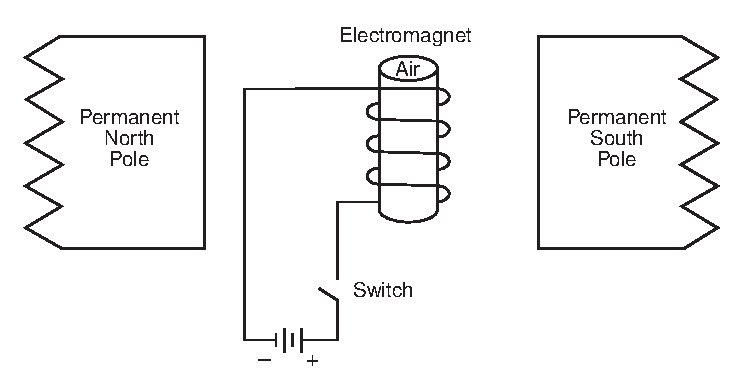
\includegraphics[keepaspectratio,scale=0.66]{June2001-Q76}
    \end{center}
    At the instant the switch is closed and a current begins
        to flow through the coil of the electromagnet,
        the coil will experience
    \begin{choices}
        %% NOTE: Positive terminal with conventional current?
        \wrongchoice{no electromagnetic force}
        \wrongchoice{a force directed out of the page}
        \wrongchoice{a counterclockwise torque}
      \correctchoice{a clockwise torque}
    \end{choices}
\end{question}
}

\element{nysed}{
\begin{question}{June2001-Q77}
    An electromagnet with an air core is located within the
        magnetic field between two permanent magnets.
    \begin{center}
        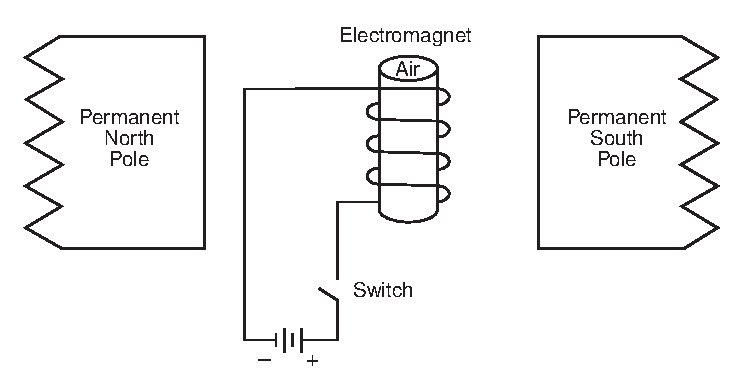
\includegraphics[keepaspectratio,scale=0.66]{June2001-Q76}
    \end{center}
    The air core of the electromagnet is replaced with an iron core.
    Compared to the strength of the magnetic field in the air core,
        the strength of the magnetic field in the iron core is
    \begin{multicols}{3}
    \begin{choices}
        \wrongchoice{less}
      \correctchoice{greater}
        \wrongchoice{the same}
    \end{choices}
    \end{multicols}
\end{question}
}

\element{nysed}{
\begin{question}{June2001-Q78}
    The two ends of a wire are connected to a galvanometer,
        forming a complete electric circuit.
    The wire is then moved through a magnetic field,
        as shown in the diagram below.
    \begin{center}
        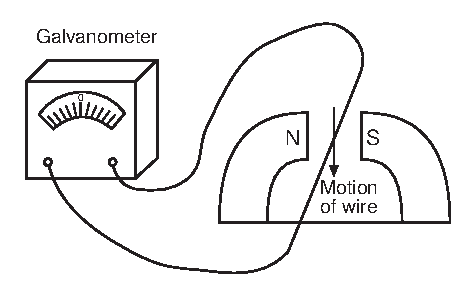
\includegraphics[keepaspectratio,scale=0.75]{June2001-Q78}
    \end{center}
    The galvanometer is being used to measure
    \begin{choices}
      \correctchoice{current}
        \wrongchoice{potential difference}
        \wrongchoice{temperature change}
        \wrongchoice{resistance}
    \end{choices}
\end{question}
}

\element{nysed}{
\begin{question}{June2001-Q79}
    Which device converts electrical energy into mechanical energy?
    \begin{multicols}{2}
    \begin{choices}
      \correctchoice{motor}
        \wrongchoice{source of emf}
        \wrongchoice{generator}
        \wrongchoice{thermocouple}
    \end{choices}
    \end{multicols}
\end{question}
}

\element{nysed}{
\begin{question}{June2001-Q80}
    The diagram below shows a point, $P$,
        located midway between two oppositely charged parallel plates.
    \begin{center}
    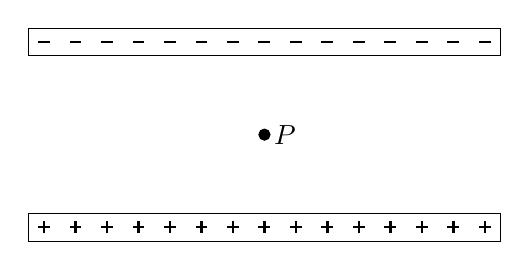
\begin{tikzpicture}
        %% Bottom
        \draw (0,0) rectangle (6,-1em);
        \foreach \x in {2,6,...,58}
            \foreach \y in {0,180}
                \draw[thick] (\x mm,2cm+0.5em) -- ++(\y:0.5ex);
        %% Top
        \draw (0,2) rectangle (6,2cm+1em);
        \foreach \x in {2,6,...,58}
            \foreach \y in {0,90,180,270}
                \draw[thick] (\x mm,-0.5em) -- ++(\y:0.5ex);
        %% Point P
        \draw[fill] (3,1.0) circle (2pt)
            node[anchor=west] {$P$};
    \end{tikzpicture}
    \end{center}
    If an electron is introduced at point $P$, the electron will
    \begin{choices}
        \wrongchoice{travel at constant speed toward the positively charged plate}
        \wrongchoice{travel at constant speed toward the negatively charged plate}
      \correctchoice{accelerate toward the positively charged plate}
        \wrongchoice{accelerate toward the negatively charged plate}
    \end{choices}
\end{question}
}

\element{nysed}{
\begin{question}{June2001-Q83}
    A potential difference of \SI{12}{\volt} is induced
        across a \SI{0.20}{\meter} long straight wire as
        it is moved at a constant speed of
        \SI{3.0}{\meter\per\second} perpendicular to a uniform magnetic field.
    What is the strength of the magnetic field?
    \begin{multicols}{2}
    \begin{choices}
        \wrongchoice{\SI{180}{\tesla}}
      \correctchoice{\SI{20}{\tesla}}
        \wrongchoice{\SI{13}{\tesla}}
        \wrongchoice{\SI{7.2}{\tesla}}
    \end{choices}
    \end{multicols}
\end{question}
}

\element{nysed}{
\begin{question}{June2001-Q84}
    A step-down transformer used to run a toy train has an
        input of \SI{120}{\volt} to its primary coil.
    A potential difference of \SI{12}{\volt} is induced in the
        secondary coil, which carries a current of \SI{12}{\ampere}.
    If the transformer operates at \SI{75}{\percent} efficiency,
        what is the current in the primary coil?
    \begin{multicols}{2}
    \begin{choices}
        \wrongchoice{\SI{0.90}{\ampere}}
      \correctchoice{\SI{1.6}{\ampere}}
        \wrongchoice{\SI{90}{\ampere}}
        \wrongchoice{\SI{160}{\ampere}}
    \end{choices}
    \end{multicols}
\end{question}
}


%% Section Jan2001
%%--------------------
\element{nysed}{
\begin{question}{Jan2001-Q76}
    Two coils of wire are wound around the same permeable core.
    Coil I has \num{200} turns and coil II has \num{3000} turns.
    Coil I is supplied with 30.0 amperes of alternating current at \SI{90.0}{\volt}.
    Which expression is a unit of potential difference equivalent to a volt?
    \begin{center}
        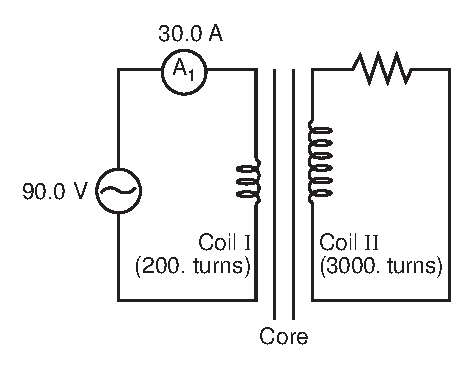
\includegraphics[keepaspectratio]{Jan2001-Q76}
    \end{center}
    What does the diagram above represent?
    \begin{choices}
        \wrongchoice{a step-up transformer}
        \wrongchoice{a step-down transformer}
        \wrongchoice{a transistor}
        \wrongchoice{an ammeter}
    \end{choices}
\end{question}
}

\element{nysed}{
\begin{question}{Jan2001-Q77}
    Two coils of wire are wound around the same permeable core.
    Coil I has \num{200} turns and coil II has \num{3000} turns.
    Coil I is supplied with \SI{30.0}{\ampere} of alternating current at \SI{90.0}{\volt}.
    Which expression is a unit of potential difference equivalent to a volt?
    \begin{center}
        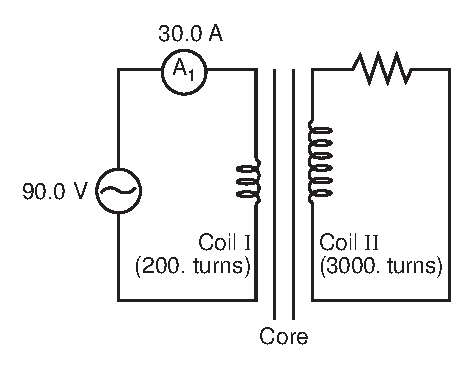
\includegraphics[keepaspectratio]{Jan2001-Q76}
    \end{center}
    What potential difference is induced in coil II?
    \begin{multicols}{2}
    \begin{choices}
        \wrongchoice{\SI{6.00}{\volt}}
        \wrongchoice{\SI{90.0}{\volt}}
      \correctchoice{\SI{1350}{\volt}}
        \wrongchoice{\SI{2700}{\volt}}
    \end{choices}
    \end{multicols}
\end{question}
}

\element{nysed}{
\begin{question}{Jan2001-Q78}
    Two coils of wire are wound around the same permeable core.
    Coil I has \num{200} turns and coil II has \num{3000} turns.
    Coil I is supplied with \SI{30.0}{\ampere} of alternating current at \SI{90.0}{\volt}.
    Which expression is a unit of potential difference equivalent to a volt?
    \begin{center}
        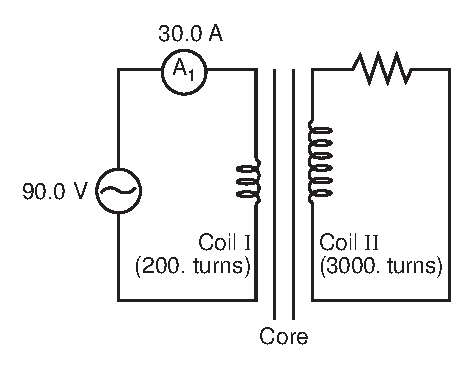
\includegraphics[keepaspectratio]{Jan2001-Q76}
    \end{center}
    What is the power developed in coil I?
    \begin{multicols}{2}
    \begin{choices}
        \wrongchoice{\SI{1.80e2}{\watt}}
      \correctchoice{\SI{2.70e3}{\watt}}
        \wrongchoice{\SI{4.05e3}{\watt}}
        \wrongchoice{\SI{4.00e2}{\watt}}
    \end{choices}
    \end{multicols}
\end{question}
}

\element{nysed}{
\begin{question}{Jan2001-Q79}
    A torque exists on the armature of an operating electric motor.
    The magnitude of this torque would decrease if there were an increase in the
    \begin{choices}
        \wrongchoice{current in the armature coil}
        \wrongchoice{magnetic field strength of the field magnet}
        \wrongchoice{potential difference applied to the armature coil}
        \wrongchoice{resistance of the wire in the armature}
    \end{choices}
\end{question}
}

\element{nysed}{
\begin{question}{Jan2001-Q80}
    In order to measure the current through an electrical device,
        an ammeter is placed in series with the device.
    Compared to the electrical device,
        the ammeter should have a much
    \begin{choices}
        \wrongchoice{lower permeability}
        \wrongchoice{higher permeability}
      \correctchoice{lower resistance}
        \wrongchoice{higher resistance}
    \end{choices}
\end{question}
}

\element{nysed}{
\begin{question}{Jan2001-Q81}
    As the armature of an operating electric motor turns,
        a voltage is induced.
    This voltage is opposite in direction to the
        applied voltage and referred to as
    \begin{multicols}{2}
    \begin{choices}
        \wrongchoice{conduction}
        \wrongchoice{reverse current}
        \wrongchoice{magnetic levitation}
        \wrongchoice{back emf}
    \end{choices}
    \end{multicols}
\end{question}
}

\element{nysed}{
\begin{question}{Jan2001-Q82}
    A voltmeter is made by connecting the current
        carrying wire loop of a galvanometer in
    \begin{choices}
        \wrongchoice{series with a high resistance}
        \wrongchoice{series with a low resistance}
        \wrongchoice{parallel with a high resistance}
        \wrongchoice{parallel with a low resistance}
    \end{choices}
\end{question}
}

\element{nysed}{
\begin{question}{Jan2001-Q83}
    The phenomenon by which an incandescent object
        gives off electrons is known as
    \begin{choices}
        \wrongchoice{thermionic emission}
        \wrongchoice{laser emission}
        \wrongchoice{induction}
        \wrongchoice{spectroscopy}
    \end{choices}
\end{question}
}

\element{nysed}{
\begin{question}{Jan2001-Q84}
    A single loop of wire is placed between the poles of permanent magnets,
        as shown in the diagram below.
    \begin{center}
        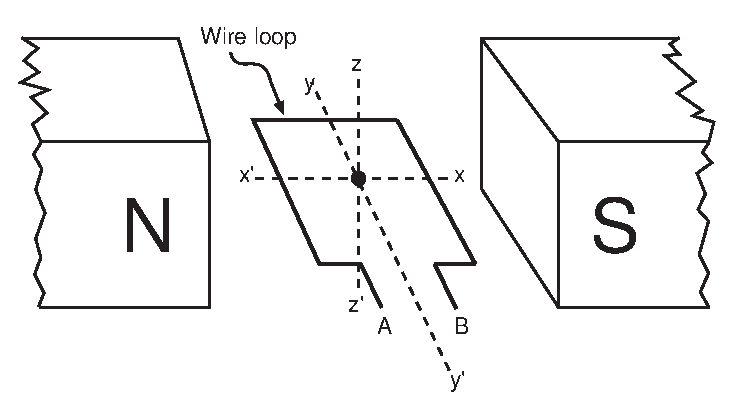
\includegraphics[width=0.95\columnwidth,keepaspectratio]{Jan2001-Q84}
    \end{center}
    If a potential difference is applied to the ends of loop AB, in which direction will the
    loop move?
    \begin{choices}
        \wrongchoice{up toward $z$}
        \wrongchoice{down toward $z'$}
        \wrongchoice{around the $y$--$y'$-axis}
        \wrongchoice{around the $x$--$x'$-axis}
    \end{choices}
\end{question}
}

\element{nysed}{
\begin{question}{Jan2001-Q85}
    The diagram below shows electron $e$ about to enter the
        region between the poles of two magnets.
    \begin{center}
        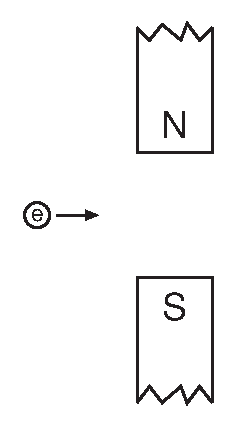
\includegraphics[scale=0.75,keepaspectratio]{Jan2001-Q85}
    \end{center}
    Upon entering the region between the poles,
        the moving electron will experience a magnetic force directed
    \begin{choices}
        \wrongchoice{toward the north pole}
        \wrongchoice{toward the south pole}
        \wrongchoice{into the page}
        \wrongchoice{out of the page}
    \end{choices}
\end{question}
}


%% Section June2000
%%--------------------
\element{nysed}{
\begin{question}{June2000-Q78}
    Which expression is a unit of potential difference equivalent to a volt?
    \begin{multicols}{2}
    \begin{choices}
        \wrongchoice{\si{\tesla\meter\per\second}}
        \wrongchoice{\si{\tesla\second\per\meter}}
      \correctchoice{\si{\tesla\meter\squared\per\second}}
        \wrongchoice{\si{\tesla\second\per\meter\squared}}
    \end{choices}
    \end{multicols}
\end{question}
}

\element{nysed}{
\begin{question}{June2000-Q76}
    A student uses identical field magnets and coils of wire,
        as well as additional components,
        to make the electric motors shown in the diagrams below.
    Which combination of core and current through the coil of wire
        will produce the greatest torque on the motor's armature?
    \begin{multicols}{2}
    \begin{choices}
        \AMCboxDimensions{down=-1.5em}
        \wrongchoice{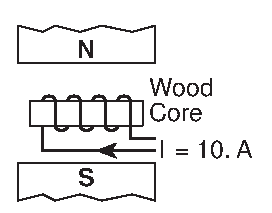
\includegraphics[keepaspectratio,scale=0.75]{June2000-Q76-A}}
        \wrongchoice{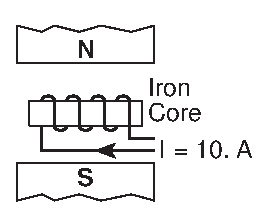
\includegraphics[keepaspectratio,scale=0.75]{June2000-Q76-B}}
        \wrongchoice{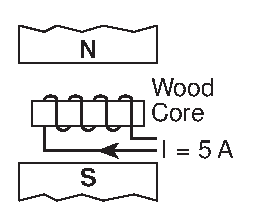
\includegraphics[keepaspectratio,scale=0.75]{June2000-Q76-C}}
        \wrongchoice{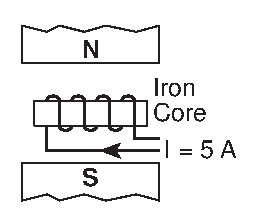
\includegraphics[keepaspectratio,scale=0.75]{June2000-Q76-D}}
    \end{choices}
    \end{multicols}
\end{question}
}

\element{nysed}{
\begin{question}{June2000-Q80}
    In a mass spectrometer,
        the strength of the magnetic field is \SI{1.0e-1}{\tesla}.
    Upon entering the chamber of the spectrometer,
        a positive ion traveling at \SI{2.0e6}{\meter\per\second}
        perpendicular to the magnetic field experiences a
        magnetic force having a magnitude of \SI{3.2e-14}{\newton}.
    The charge on this positive ion is
    \begin{multicols}{2}
    \begin{choices}
        \wrongchoice{\SI{6.4e-21}{\coulomb}}
      \correctchoice{\SI{1.6e-19}{\coulomb}}
        \wrongchoice{\SI{6.4e-9}{\coulomb}}
        \wrongchoice{\SI{1.6e-9}{\coulomb}}
    \end{choices}
    \end{multicols}
\end{question}
}

\element{nysed}{
\begin{question}{June2000-Q81}
    The Millikan oil drop experiment was designed to
        determine the
    \begin{choices}
        \wrongchoice{sign of the charge of an electron}
        \wrongchoice{mass of a proton}
        \wrongchoice{ratio of charge to mass of an electron}
      \correctchoice{magnitude of the charge of an electron}
    \end{choices}
\end{question}
}

\element{nysed}{
\begin{question}{June2000-Q82}
    A transformer plugged into a \SI{120}{\volt} household electrical outlet is used to operate a doorbell at a potential difference of \SI{12}{\volt}.
    What is the ratio of the number of turns in the primary coil to the number of turns in the secondary coil of the transformer?
    %% TODO: Check this
    \begin{multicols}{2}
    \begin{choices}
        \wrongchoice{$10:1$}
        \wrongchoice{$12:1$}
        \wrongchoice{$120:1$}
        \wrongchoice{$1440:1$}
    \end{choices}
    \end{multicols}
\end{question}
}

\element{nysed}{
\begin{question}{June2000-Q83}
    The diagram below shows an evacuated cathode ray tube consisting of a source of electrons at one end,
        a fluorescent screen at the other end,
        and a pair of oppositely charged parallel plates in between.
    \begin{center}
        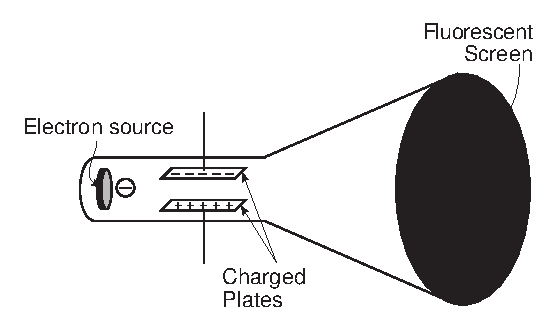
\includegraphics[keepaspectratio,scale=0.75]{June2000-Q83}
    \end{center}
    Which diagram best represents the motion of the electron beam in the tube as it passes between the oppositely charged plates?
    \begin{multicols}{2}
    \begin{choices}
        \AMCboxDimensions{down=-2.5em}
      \correctchoice{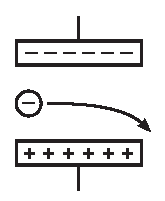
\includegraphics[keepaspectratio,scale=0.85]{June2000-Q83-A}}
        \wrongchoice{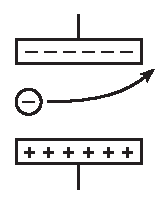
\includegraphics[keepaspectratio,scale=0.85]{June2000-Q83-B}}
        \wrongchoice{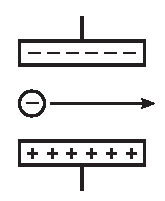
\includegraphics[keepaspectratio,scale=0.85]{June2000-Q83-C}}
        \wrongchoice{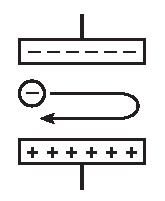
\includegraphics[keepaspectratio,scale=0.85]{June2000-Q83-D}}
    \end{choices}
    \end{multicols}
\end{question}
}

\element{nysed}{
\begin{question}{June2000-Q84}
    In the diagram below, a potential difference is
        induced in a rectangular wire loop as it is rotated
        at constant speed between two magnetic poles.
    \begin{center}
        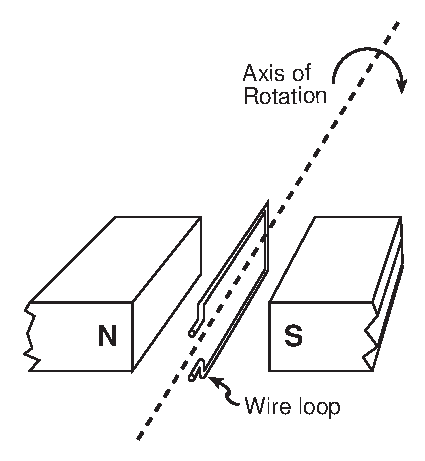
\includegraphics[keepaspectratio]{June2000-Q84}
    \end{center}
    If the direction of the field is reversed and the speed
        of rotation is doubled, the magnitude of the maximum
        induced potential difference will be
    \begin{multicols}{2}
    \begin{choices}
        \wrongchoice{one-half as great}
        \wrongchoice{the same}
      \correctchoice{twice as great}
        \wrongchoice{four times as great}
    \end{choices}
    \end{multicols}
\end{question}
}

\element{nysed}{
\begin{question}{June2000-Q85}
    A \SI{100}{\percent} efficient transformer has \num{40}
        turns of wire in the primary coil and \num{80}
        turns of wire in the secondary coil.
    If \SI{20}{\watt} of power is supplied to the primary coil,
        the power developed in the secondary coil will be
    \begin{multicols}{2}
    \begin{choices}
        \wrongchoice{\SI{10}{\watt}}
      \correctchoice{\SI{20}{\watt}}
        \wrongchoice{\SI{80}{\watt}}
        \wrongchoice{\SI{160}{\watt}}
    \end{choices}
    \end{multicols}
\end{question}
}

%% Section June1999
%%--------------------
\element{nysed}{
\begin{question}{June1999-Q76}
    Which graph best represents the relationship between the deflection
        of a galvanometer coil and the current passing through the coil?
    \begin{multicols}{2}
    \begin{choices}
        \AMCboxDimensions{down=-2.5em}
        \correctchoice{
            \begin{tikzpicture}
                \begin{axis}[
                    axis y line=left,
                    axis x line=bottom,
                    axis line style={->},
                    xlabel={current},
                    xtick=\empty,
                    ylabel={deflection},
                    ytick=\empty,
                    xmin=0,xmax=11,
                    ymin=0,ymax=11,
                    width=\columnwidth,
                    very thin,
                ]
                \addplot[line width=1pt,domain=0:10]{x};
                \end{axis}
            \end{tikzpicture}
        }
        \wrongchoice{
            \begin{tikzpicture}
                \begin{axis}[
                    axis y line=left,
                    axis x line=bottom,
                    axis line style={->},
                    xlabel={current},
                    xtick=\empty,
                    ylabel={deflection},
                    ytick=\empty,
                    xmin=0,xmax=11,
                    ymin=0,ymax=11,
                    width=\columnwidth,
                    very thin,
                ]
                \addplot[line width=1pt,domain=0:10]{10/x};
                \end{axis}
            \end{tikzpicture}
        }
        \wrongchoice{
            \begin{tikzpicture}
                \begin{axis}[
                    axis y line=left,
                    axis x line=bottom,
                    axis line style={->},
                    xlabel={current},
                    xtick=\empty,
                    ylabel={deflection},
                    ytick=\empty,
                    xmin=0,xmax=11,
                    ymin=0,ymax=11,
                    width=\columnwidth,
                    very thin,
                ]
                \addplot[line width=1pt,domain=0:10]{8};
                \end{axis}
            \end{tikzpicture}
        }
        \wrongchoice{
            \begin{tikzpicture}
                \begin{axis}[
                    axis y line=left,
                    axis x line=bottom,
                    axis line style={->},
                    xlabel={current},
                    xtick=\empty,
                    ylabel={deflection},
                    ytick=\empty,
                    xmin=0,xmax=11,
                    ymin=0,ymax=11,
                    width=\columnwidth,
                    very thin,
                ]
                \addplot[line width=1pt,domain=0:10]{0.1 *x *x};
                \end{axis}
            \end{tikzpicture}
        }
    \end{choices}
    \end{multicols}
\end{question}
}

\element{nysed}{
\begin{question}{June1999-Q77}
    A positively charged particle traveling at \SI{7.5e5}{\meter\per\second}
        enters a uniform magnetic field perpendicular to the lines of force.
    While in the \SI{4.0e-2}{\tesla} magnetic field,
        a net force of \SI{9.6e-15}{\newton} acts on the particle.
    What is the magnitude of the charge on the particle?
    \begin{multicols}{2}
    \begin{choices}
        \wrongchoice{\SI{1.6e-19}{\coulomb}}
      \correctchoice{\SI{3.2e-19}{\coulomb}}
        \wrongchoice{\SI{9.6e-19}{\coulomb}}
        \wrongchoice{\SI{3.2e-19}{\coulomb}}
    \end{choices}
    \end{multicols}
\end{question}
}

\element{nysed}{
\begin{question}{June1999-Q78}
    What did Millikan conclude after performing his oil-drop experiment?
    \begin{choices}
        \wrongchoice{The charge on an electron is \SI{1.0}{\coulomb}}
        \wrongchoice{The mass of an electron is \SI{1.7e-27}{\kilo\gram}}
      \correctchoice{The charge on any oil drop is an integral multiple of the charge on an electron.}
        \wrongchoice{The charge on any oil drop may have any value larger than \SI{1.6e-19}{\coulomb}.}
    \end{choices}
\end{question}
}

\element{nysed}{
\begin{question}{June1999-Q79}
    A high-resistance wire is connected in series with the coil of a galvanometer.
    The function of the high-resistance wire is to:
    \begin{choices}
      \correctchoice{limit the current in the coil}
        \wrongchoice{prevent a potential drop across the coil}
        \wrongchoice{allow the modified meter to get warm.}
        \wrongchoice{decrease the internal temperature of the modified galvanometer}
    \end{choices}
\end{question}
}

\element{nysed}{
\begin{question}{June1999-Q80}
    An electromagnetic device used to determine the masses of individual atoms is:
    \begin{choices}
        \wrongchoice{an induction coil}
        \wrongchoice{an electroscope}
        \wrongchoice{a galvanometer}
      \correctchoice{a mass spectrometer}
    \end{choices}
\end{question}
}

\element{nysed}{
\begin{question}{June1999-Q81}
    In the diagram below, a segment of wire, $RS$, which is \SI{0.20}{\meter} in length,
        is free to slide along a U-shaped wire located in a uniform \SI{0.60}{\tesla} magnetic field directed into the page.
    \begin{center}
    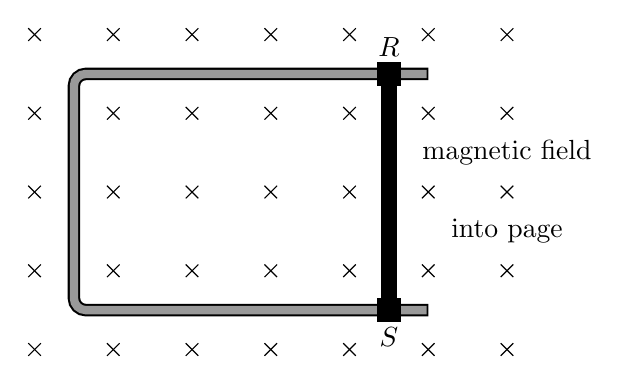
\begin{tikzpicture}
        %% magnetic field into page
        \foreach \x in {0,1,2,3,4,5,6}
            \foreach \y in {-2,-1,0,1,2}
                \foreach \z in {45,135,225,315}
                    \draw[thin]  (\x,\y) -- ++(\z:0.75ex);
        \node[anchor=center] at (6,+0.5)  {magnetic field};
        \node[anchor=center] at (6,-0.5)  {into page};
        %% U-shaped Bar
        \draw[line width=4.5pt,rounded corners=1ex] (5,1.5) -- (0.5,1.5) -- (0.5,-1.5) -- (5,-1.5); 
        \draw[line width=3.0pt,rounded corners=1ex,white!60!black] (4.98,1.5) -- (0.5,1.5) -- (0.5,-1.5) -- (4.98,-1.5); 
        %% Nodes R
        \node[anchor=south] at (4.5,1.6) {$R$};
        \fill (4.35,1.65) rectangle (4.65,1.35);
        %% Nodes S
        \node[anchor=north] at (4.5,-1.6) {$S$};
        \fill (4.35,-1.65) rectangle (4.65,-1.35);
        %% Bar RS
        \fill (4.4,1.4) rectangle (4.6,-1.4);
    \end{tikzpicture}
    \end{center}
    If the wire segment $RS$ is slid to the right at a constant speed of \SI{4.0}{\meter\per\second},
        the potential difference induced across the ends of the wire segment is:
    \begin{multicols}{2}
    \begin{choices}
        \wrongchoice{\SI{0.12}{\volt}}
      \correctchoice{\SI{0.48}{\volt}}
        \wrongchoice{\SI{2.4}{\volt}}
        \wrongchoice{\SI{4.8}{\volt}}
    \end{choices}
    \end{multicols}
\end{question}
}

\element{nysed}{
\begin{question}{June1999-Q82}
    A direct-current source is used to operate an electric motor.
    After each half-rotation of the armature, the split ring commutator
    \begin{choices}
        \wrongchoice{reverses the direction of the field magnet}
        \wrongchoice{increases the strength of the field magnet}
      \correctchoice{reverses the direction of the current in the armature}
        \wrongchoice{increases the current in the armature}
    \end{choices}
\end{question}
}

\element{nysed}{
\begin{question}{June1999-Q83}
    In order for a transformer to function, its primary and secondary coils must
    \begin{choices}
        \wrongchoice{be made of different elements}
        \wrongchoice{be kept at different temperatures}
        \wrongchoice{have the same weight}
      \correctchoice{have continually changing magnetic fields}
    \end{choices}
\end{question}
}

\element{nysed}{
\begin{question}{June1999-Q84}
    A \SI{100}{\percent} efficient transformer has an \num{800} turn
        primary coil connected to a \SI{120}{\volt} alternating current source.
    If the secondary coil has \num{400} turns,
        what is the voltage induced in the secondary coil?
    \begin{multicols}{2}
    \begin{choices}
        \wrongchoice{\SI{30}{\volt}}
      \correctchoice{\SI{60}{\volt}}
        \wrongchoice{\SI{240}{\volt}}
        \wrongchoice{\SI{480}{\volt}}
    \end{choices}
    \end{multicols}
\end{question}
}

\element{nysed}{
\begin{question}{June1999-Q85}
    An electron is located between two oppositively charged parallel plates as shown in the diagram below.
    \begin{center}
    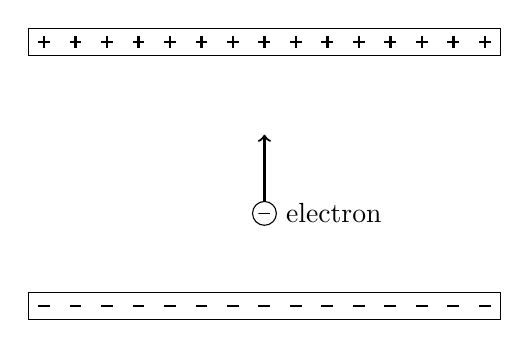
\begin{tikzpicture}
        %% electron
        \draw[thick,->] (3,1) -- (3,2);
        \draw[fill=white] (3,1) circle (1ex) node[anchor=west,xshift=1ex] {electron};
        \draw (3,1) -- ++(180:0.5ex) -- ++(0:1ex);
        %% Bottom negative
        \draw (0,0) rectangle (6,-1em);
        \foreach \x in {2,6,...,58}
            \foreach \y in {0,180} {
                \draw[thick] (\x mm,-0.5em) -- ++(\y:0.5ex);
            }
        %% Top positive
        \draw (0,3) rectangle (6,3cm+1em);
        \foreach \x in {2,6,...,58}
            \foreach \y in {0,90,180,270} {
                \draw[thick] (\x mm,3cm+0.5em) -- ++(\y:0.5ex);
            }
    \end{tikzpicture}
    \end{center}
    As the electron moves toward the positive plate,
        the magnitude of the electric force acting on the electron
    \begin{multicols}{2}
    \begin{choices}
        \wrongchoice{decreases}
        \wrongchoice{increases}
      \correctchoice{remains the same}
    \end{choices}
    \end{multicols}
\end{question}
}


%% Section June1998
%%--------------------
\element{nysed}{
\begin{question}{June1998-Q76}
    In the diagram below,
        a free electron is traveling upward at speed $v$ parallel to a conductor.
    An electron current begins to flow upward in the conductor.
    \begin{center}
    \begin{tikzpicture}
        %% NOTE: TODO:  draw tikz
    \end{tikzpicture}
    \end{center}
    Which diagram best represents the resulting magnetic field, $B$,
        and the direction of the magnetic force, $F$, on the free electron?
    \begin{multicols}{2}
    \begin{choices}
        \wrongchoice{
            \begin{tikzpicture}
            \end{tikzpicture}
        }
    \end{choices}
    \end{multicols}
\end{question}
}

\element{nysed}{
\begin{question}{June1998-Q77}
    A magnetic force acts on a charged particle moving at a constant speed perpendicular to a uniform magnetic field.
    The magnitude of the magnetic force on the particle will increase if the:
    \begin{choices}
      \correctchoice{flux density of the magnetic field increases}
        \wrongchoice{time of travel of the charge increases}
        \wrongchoice{magnitude of the charge decreases}
        \wrongchoice{speed of the charge decreases}
    \end{choices}
\end{question}
}

\element{nysed}{
\begin{question}{June1998-Q78}
    Which statement best describes the torque experiences by a current-carrying loop of wire in an external magnetic field?
    \begin{choices}
        \wrongchoice{It is due to the current in the loop of wire, only}
      \correctchoice{It is due to the interaction of the external magnetic field and the magnetic field produced by current in the loop.}
        \wrongchoice{It is inversely proportional to the length of the conducting loop in the magnetic field.}
        \wrongchoice{It is inversely proportional to the strength of the permanent magnetic field.}
    \end{choices}
\end{question}
}

\element{nysed}{
\begin{question}{June1998-Q79}
    Which device consists of a galvanometer with a low-resistance shunt placed in parallel across its terminals?
    \begin{multicols}{2}
    \begin{choices}
        \wrongchoice{mass spectrometer}
        \wrongchoice{transformer}
        \wrongchoice{voltmeter}
      \correctchoice{ammeter}
    \end{choices}
    \end{multicols}
\end{question}
}

\element{nysed}{
\begin{question}{June1998-Q80}
    An operating electric motor produces a back emf,
        which opposes the applied potential difference.
    As a result, the armature current:
    \begin{choices}
      \correctchoice{decreases}
        \wrongchoice{increases}
        \wrongchoice{changed from d.c. to a.c.}
        \wrongchoice{changed from a.c. to d.c.}
    \end{choices}
\end{question}
}

\element{nysed}{
\begin{question}{June1998-Q81}
    As the temperature of a surface increases,
        how does the rate of thermionic emission change?
    \begin{choices}
        \wrongchoice{Electrons are emitted at a lower rate.}
      \correctchoice{Electrons are emitted at a higher rate.}
        \wrongchoice{Protons are emitted at a lower rate.}
        \wrongchoice{Protons are emitted at a higher rate.}
    \end{choices}
\end{question}
}

\element{nysed}{
\begin{question}{June1998-Q82}
    In an operating mass spectrometer,
        the motion of positive ion beams is influenced by:
    \begin{choices}
        \wrongchoice{electric fields, only}
        \wrongchoice{magnetic fields, only}
      \correctchoice{both electric and magnetic fields}
        \wrongchoice{neither electric nor magnetic fields}
    \end{choices}
\end{question}
}

\element{nysed}{
\begin{question}{June1998-Q83}
    The diagram below, which illustrates the Millikan oil drop experiment,
        shows a \SI{3.2e-14}{\kilo\gram} oil drop with a charge of \SI{-1.6e-18}{\coulomb}.
    The oil drop was in equilibrium when the upward electric force on the drop was equal in magnitude to the gravitational force on the drop.
    \begin{center}
    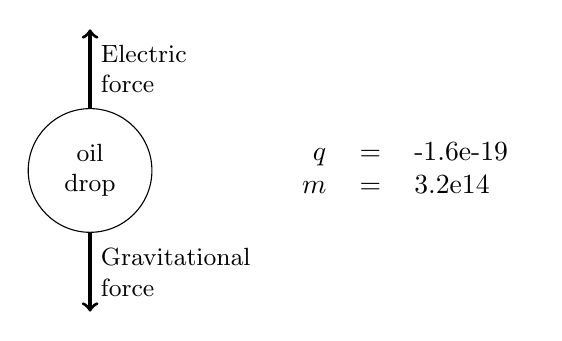
\begin{tikzpicture}
        \begin{scope}[xshift=-2cm,font=\small]
            \node[circle,draw,text width=3em,text centered] (A) at (0,0) {oil drop};
            \draw[very thick,->] (A.north) -- ++(90:1) node[pos=0.5,anchor=west,text width=4em] {Electric force};
            \draw[very thick,->] (A.south) -- ++(270:1) node[pos=0.5,anchor=west,text width=6em] {Gravitational force};
        \end{scope}
        \begin{scope}[xshift=+2cm]
            \node[anchor=center] at (0,0) {
                \begin{tabular}{rcl}
                    $q$ & = & \SI{-1.6e-19}{\coulomb} \\
                    $m$ & = & \SI{3.2e14}{\kilo\gram} \\
                \end{tabular}
                };
        \end{scope}
    \end{tikzpicture}
    \end{center}
    What was the magnitude of the electric field intensity when this oil drop was in equilibrium?
    \begin{multicols}{2}
    \begin{choices}
        \wrongchoice{\SI{2.0e-5}{\newton\per\coulomb}}
      \correctchoice{\SI{2.0e5}{\newton\per\coulomb}}
        \wrongchoice{\SI{5.0e-5}{\newton\per\coulomb}}
        \wrongchoice{\SI{5.0e5}{\newton\per\coulomb}}
    \end{choices}
    \end{multicols}
\end{question}
}

\element{nysed}{
\begin{question}{June1998-Q84}
    The diagram below shows an end view of a metal rod moving upward perpendicular to a uniform magnetic field having a flux density of \SI{2.0e-2}{\tesla}.
    The \SI{2.0}{\meter} long wire is moving at a constant speed of \SI{3.0}{\meter\per\second}.
    \begin{center}
    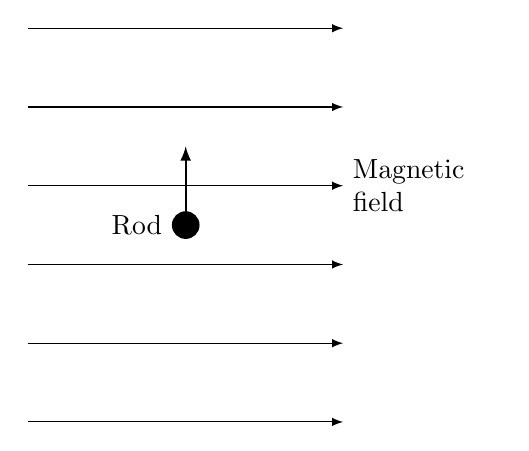
\begin{tikzpicture}
        %% magnetic field
        \foreach \y in {-25,-15,...,25} \draw[-latex] (-2,\y mm) -- (2,\y mm);
        \node[anchor=west,text width=5em] at (2,0.5) {Magnetic field};
        %% Rod
        \draw[thick,-latex] (0,0) -- (0,1);
        \fill (0,0) circle (5pt);
        \node[anchor=east] at (-5pt,0) {Rod};
    \end{tikzpicture}
    \end{center}
    What is the emf induced across the rod?
    \begin{multicols}{2}
    \begin{choices}
        \wrongchoice{\SI{0.060}{\volt}}
      \correctchoice{\SI{0.12}{\volt}}
        \wrongchoice{\SI{1.2}{\volt}}
        \wrongchoice{\SI{6.0}{\volt}}
    \end{choices}
    \end{multicols}
\end{question}
}

\element{nysed}{
\begin{question}{June1998-Q85}
    The diagram below shows a step-up transformer having a primary coil with two windings and a secondary coil with four windings.
    \begin{center}
    \begin{tikzpicture}
        %% NOTE: TODO: draw tikz
    \end{tikzpicture}
    \end{center}
    When a potential difference of \SI{12}{\volt} is applied to the primary coil,
        what is the current in an \SI{8.0}{\ohm} resistor connected to the secondary coil as shown?
    \begin{multicols}{2}
    \begin{choices}
        \wrongchoice{\SI{0.33}{\ampere}}
        \wrongchoice{\SI{0.75}{\ampere}}
      \correctchoice{\SI{3.0}{\ampere}}
        \wrongchoice{\SI{4.5}{\ampere}}
    \end{choices}
    \end{multicols}
\end{question}
}


%% Section June1997
%%--------------------
\element{nysed}{
\begin{question}{June1997-Q76}
    A high resistance is connected in series with the internal coil of a galvanometer to make:
    \begin{multicols}{2}
    \begin{choices}
        \wrongchoice{A motor}
        \wrongchoice{an ammeter}
      \correctchoice{a voltmeter}
        \wrongchoice{a generator}
    \end{choices}
    \end{multicols}
\end{question}
}

\element{nysed}{
\begin{question}{June1997-Q77}
    A student uses a voltmeter to measure the potential difference across a circuit resistor.
    To obtain a correct reading,
        the student must connect the voltmeter:
    \begin{choices}
      \correctchoice{in parallel with the circuit resistor}
        \wrongchoice{in series with the circuit resistor}
        \wrongchoice{before connecting the other circuit components}
        \wrongchoice{after connecting the other circuit components}
    \end{choices}
\end{question}
}

\newcommand{\nysedJuneNineteenNinetySevenQSeventyEight}{
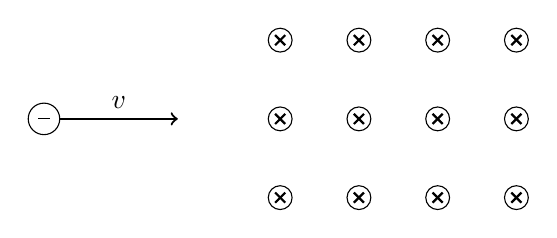
\begin{tikzpicture}
    %% B field into page
    \foreach \x in {0,10,...,30}
        \foreach \y in {-10,0,10} {
            \draw[thin] (\x mm,\y mm) circle (1ex);
            \foreach \z in {45,135,225,315}
                \draw[thick] (\x mm,\y mm) -- ++ (\z:0.6ex);
        }
    %% electron
    \draw (-3,0) -- ++(180:0.5ex) -- ++(0:1ex);
    \draw (-3,0) circle (0.2);
    \draw[thick,->] (-2.8,0) -- ++(0:1.5) node[pos=0.5,anchor=south] {$v$};
\end{tikzpicture}
}

\element{nysed}{
\begin{question}{June1997-Q78}
    The diagram below represents an electron moving with speed $v$ to the right and about to enter a uniform magnetic field acting into the page.
    \begin{center}
        \nysedJuneNineteenNinetySevenQSeventyEight
    \end{center}
    Upon entering the magnetic field,
        the electron will be deflected:
    \begin{choices}
        \wrongchoice{into the page}
        \wrongchoice{out the page}
        \wrongchoice{toward the top of the page}
      \correctchoice{toward the bottom of the page}
    \end{choices}
\end{question}
}

\element{nysed}{
\begin{question}{June1997-Q79}
    The diagram below represents an electron moving with speed $v$ to the right and about to enter a uniform magnetic field acting into the page.
    \begin{center}
        \nysedJuneNineteenNinetySevenQSeventyEight
    \end{center}
    If the speed of the electron is \SI{3.0e3}{\meter\per\second} and the magnitude of the magnetic field is \SI{3.0e-5}{\tesla},
        the magnitude of the magnetic force on the electron is approximately:
    \begin{multicols}{2}
    \begin{choices}
        \wrongchoice{\SI{4.8e-24}{\newton}}
      \correctchoice{\SI{1.4e-20}{\newton}}
        \wrongchoice{\SI{4.8e-16}{\newton}}
        \wrongchoice{\SI{9.0e-2}{\newton}}
    \end{choices}
    \end{multicols}
\end{question}
}

\element{nysed}{
\begin{question}{June1997-Q80}
    In a transformer, two coils of wire are wound around a common iron core.
    To operate properly, the transformer requires:
    \begin{choices}
      \correctchoice{an alternating-current source connected to the primary coil}
        \wrongchoice{an direct-current source connected to the primary coil}
        \wrongchoice{more turns in the primary coil than in the secondary coil}
        \wrongchoice{more turns in the secondary coil than in the primary coil}
    \end{choices}
\end{question}
}

\element{nysed}{
\begin{question}{June1997-Q81}
    Two hollow core solenoids, $A$ and $B$, are connected by a wire,
        as shown in the diagram below.
    Two bar magnets, 1 and 2, are suspended just above the solenoids.
    \begin{center}
    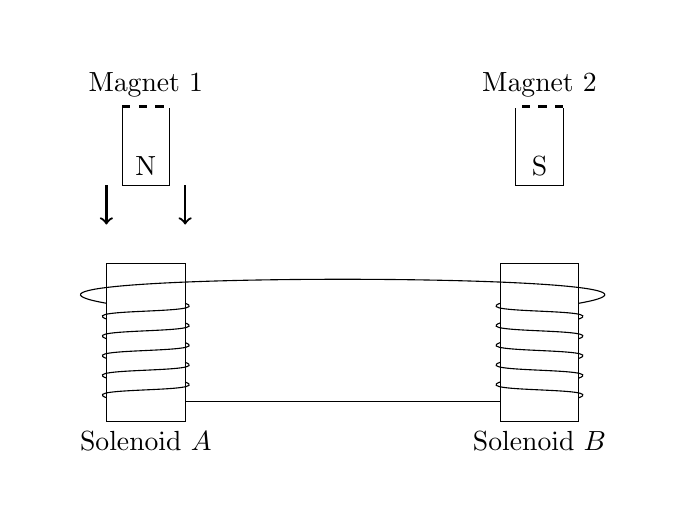
\begin{tikzpicture}
        \clip (-4,-3) rectangle (4,3);
        %% solenoid A
        \draw (-3,-2) rectangle (-2,0);
        \node[ anchor=north] at (-2.5,-2) {Solenoid $A$};
        %% solenoid B
        \draw (+3,-2) rectangle (+2,0);
        \node[ anchor=north] at (+2.5,-2) {Solenoid $B$};
        %% Wires
        \draw (-3,-0.5) to[out=170,in=10,tension=0] (3,-0.5);
        \draw (-2,-1.75) -- (2,-1.75);
        \foreach \x in {-0.5,-0.75,-1.0,-1.25,-1.5} {
            \draw (-2,\x) to[out=340,in=160] (-3,{\x-0.2});
            \draw (+2,\x) to[out=200,in=20] (+3,{\x-0.2});
        }
        %% magnet 1
        \node[anchor=south] at (-2.5,2) {Magnet 1};
        \draw (-2.80,2) rectangle (-2.2,1);
        \draw[white,thick] (-3,2) -- (-2,2);
        \draw[dashed,thick] (-2.8,2) -- (-2.2,2);
        \node[anchor=south] at (-2.5,1) {N};
        \draw[thick,->] (-3,1) -- (-3,0.5);
        \draw[thick,->] (-2,1) -- (-2,0.5);
        %% magnet 2
        \node[anchor=south] at (+2.5,2) {Magnet 2};
        \draw (+2.80,2) rectangle (+2.2,1);
        \draw[white,thick] (+3,2) -- (+2,2);
        \draw[dashed,thick] (+2.8,2) -- (+2.2,2);
        \node[anchor=south] at (+2.5,1) {S};
    \end{tikzpicture}
    \end{center}
    If the north pole of magnet 1 is dropped through solenoid $A$,
        the south pole of magnet 2 will simultaneously be:
    \begin{choices}
      \correctchoice{attracted by a magnetic force toward solenoid $B$}
        \wrongchoice{repelled by a magnetic force toward solenoid $B$}
        \wrongchoice{repelled by an electric force away from solenoid $B$}
        \wrongchoice{unaffected by solenoid $B$}
    \end{choices}
\end{question}
}

\element{nysed}{
\begin{question}{June1997-Q82}
    Which device can be used to increase the voltage from a source of direct current?
    \begin{multicols}{2}
    \begin{choices}
        \wrongchoice{electroscope}
        \wrongchoice{mass spectrometer}
      \correctchoice{induction coil}
        \wrongchoice{generator}
    \end{choices}
    \end{multicols}
\end{question}
}

\element{nysed}{
\begin{question}{June1997-Q83}
    The graph below shows induced potential difference
        verses time for the rotating armature of a generator.
    \begin{center}
    \begin{tikzpicture}
        \begin{axis}[
            axis y line=left,
            axis x line=middle,
            axis line style={->},
            xlabel={time},
            x unit=\SI{e-2}{\second},
            xtick={0,0.05,0.10},
            xticklabels={0,5,10},
            ylabel={potential},
            y unit=\si{\volt},
            ytick={-120,0,120},
            xmin=0,xmax=0.11,
            ymin=-130,ymax=130,
            width=0.8\columnwidth,
            height=0.5\columnwidth,
            very thin,
        ]
        \addplot[line width=1pt,domain=0:0.1,samples=50]{120*sin(7200*x)};
        \end{axis}
    \end{tikzpicture}
    \end{center}
    What is the frequency of armature rotation?
    \begin{multicols}{2}
    \begin{choices}
        \wrongchoice{\SI{10}{\hertz}}
      \correctchoice{\SI{20}{\hertz}}
        \wrongchoice{\SI{40}{\hertz}}
        \wrongchoice{\SI{60}{\hertz}}
    \end{choices}
    \end{multicols}
\end{question}
}

\element{nysed}{
\begin{question}{June1997-Q84}
    The transformer on a power pole steps down the voltage from \SI{10 800}{\volt} to \SI{120}{\volt}.
    If the secondary coil contains \num{360} turns,
        how many turns are in the primary coil?
    \begin{multicols}{2}
    \begin{choices}
        \wrongchoice{\num{30}}
        \wrongchoice{\num{90}}
        \wrongchoice{\num{3600}}
      \correctchoice{\num{32 400}}
    \end{choices}
    \end{multicols}
\end{question}
}

\element{nysed}{
\begin{question}{June1997-Q85}
    An electron is located between a pair of oppositely charged parallel plates.
    As the electron approaches the positive plate,
        the kinetic energy of the electron:
    \begin{multicols}{2}
    \begin{choices}
        \wrongchoice{decreases}
      \correctchoice{increases}
        \wrongchoice{remains the same}
    \end{choices}
    \end{multicols}
\end{question}
}


%% Section June1996
%%--------------------
\element{nysed}{
\begin{question}{June1996-Q76}
    Which diagram best represents how galvanometer $G$ can be modified to make it a voltmeter?
    [In the diagrams, $R$ represents resistance.]
    \begin{multicols}{2}
    \begin{choices}\small
        \AMCboxDimensions{down=-1.4cm}
        \ctikzset{bipoles/length=0.75cm}
        \wrongchoice{
            \begin{circuitikz}
                \draw[white] (-0.1,0) -- (3.1,0);
                \fill (0,0) circle (2pt); \fill (3,0) circle (2pt);
                \draw (0,0) to (0,1) to [R,l={High $R$}] (3,1) to (3,0);
                \draw (0,1) to (0,3) to (3,3) to (3,1);
                \node[draw,circle,fill=white,anchor=center] at (1.5,3) {$G$};
            \end{circuitikz}
        }
        \wrongchoice{
            \begin{circuitikz}
                \draw[white] (-0.1,0) -- (3.1,0);
                \fill (0,0) circle (2pt); \fill (3,0) circle (2pt);
                \draw (0,0) to[*-] (0,1) to [R,l={Low $R$}] (3,1) to (3,0);
                \draw (0,1) to (0,3) to (3,3) to (3,1);
                \node[draw,circle,fill=white,anchor=center] at (1.5,3) {$G$};
            \end{circuitikz}
        }
        \correctchoice{
            \begin{circuitikz}
                \draw[white] (-0.1,0) -- (3.1,0);
                \fill (0,0) circle (2pt); \fill (3,0) circle (2pt);
                \draw (0,0) to [R,l_={High $R$}] (0,3) to (3,3) to (3,0);
                \node[draw,circle,fill=white,anchor=center] at (1.5,3) {$G$};
            \end{circuitikz}
        }
        \wrongchoice{
            \begin{circuitikz}
                \draw[white] (-0.1,0) -- (3.1,0);
                \fill (0,0) circle (2pt); \fill (3,0) circle (2pt);
                \draw (0,0) to [R,l_={Low $R$}] (0,3) to (3,3) to (3,0);
                \node[draw,circle,fill=white,anchor=center] at (1.5,3) {$G$};
            \end{circuitikz}
        }
    \end{choices}
    \end{multicols}
\end{question}
}

\element{nysed}{
\begin{question}{June1996-Q77}
    A motor is to rotational mechanical energy as a generator is to:
    \begin{choices}
        \wrongchoice{chemical potential energy}
      \correctchoice{induced electrical energy}
        \wrongchoice{thermal internal energy}
        \wrongchoice{elastic potential energy}
    \end{choices}
\end{question}
}

\element{nysed}{
\begin{question}{June1996-Q78}
    A split-ring commutator is used to:
    \begin{choices}
        \wrongchoice{reduce the voltage in a transformer}
        \wrongchoice{reduce the resistance of a shunt in an ammeter}
        \wrongchoice{make the light waves coherent in a laser}
      \correctchoice{keep the torque acting in the same direction}
    \end{choices}
\end{question}
}

\element{nysed}{
\begin{question}{June1996-Q79}
    A straight conductor \SI{1.0}{\meter} long is moved at a constant speed of \SI{10}{\meter\per\second} perpendicular to a magnetic field.
    If the flux density of the field is \SI{5.0e-3}{\tesla},
        what is the magnitude of the electromotive force induced in the conductor?
    \begin{multicols}{2}
    \begin{choices}
        \wrongchoice{\SI{0.0}{\volt}}
        \wrongchoice{\SI{2.0e3}{\volt}}
      \correctchoice{\SI{5.0e-2}{\volt}}
        \wrongchoice{\SI{5.0e-4}{\volt}}
    \end{choices}
    \end{multicols}
\end{question}
}

\newcommand{\JuneOneNineNineSixQEighty}{
\begin{tikzpicture}
    %% left positive
    \draw (-1em,0) rectangle (0,-3);
    \foreach \x in {2,6,...,28}
        \foreach \y in {0,90,180,270} {
            \draw[thick] (-0.5em,-\x mm) -- ++(\y:0.5ex);
        }
    %% right negative
    \draw (2,0) rectangle (2cm+1em,-3);
    \foreach \x in {2,6,...,28}
        \foreach \y in {0,180} {
            \draw[thick] (2cm+0.5em,-\x mm) -- ++(\y:0.5ex);
        }
    %% electron
    \foreach \y in {0,90,180,270} \draw[thick] (1,1) -- ++(\y:0.5ex);
    \draw (1,1) circle (1ex) node[anchor=west,xshift=1ex] {e};
    \draw[thick,->] (1,1cm-1ex) -- (1,0);
\end{tikzpicture}
}

\element{nysed}{
\begin{question}{June1996-Q80}
    The diagram below represents an electron being projected between two oppositely charged parallel plates.
    \begin{center}
        \JuneOneNineNineSixQEighty
    \end{center}
    In which direction will the electric field deflect the electron?
    \begin{multicols}{2}
    \begin{choices}
        \wrongchoice{into the page}
        \wrongchoice{out of the page}
        \wrongchoice{to the right}
      \correctchoice{to the left}
    \end{choices}
    \end{multicols}
\end{question}
}

\element{nysed}{
\begin{question}{June1996-Q81}
    The diagram below represents an electron being projected between two oppositely charged parallel plates.
    \begin{center}
        \JuneOneNineNineSixQEighty
    \end{center}
    As an electron moves through an electric field,
        the magnitude of the electric force on the electron:
    \begin{choices}
        \wrongchoice{decreases}
        \wrongchoice{increases}
      \correctchoice{remains the same}
    \end{choices}
\end{question}
}

\element{nysed}{
\begin{question}{June1996-Q82}
    The diagram below represents a negatively charged oil drop between two oppositely charged parallel plates.
    The forces acting on the oild drop are in equilibrium.
    \begin{center}
    \begin{circuitikz}
        %% circuit
        \draw (0,0) to [battery,v] (0,3)  to (4,3) to (4,2.6);
        \draw (0,0) to (4,0) to (4,0.4);
        %% charged plates
        \draw[thick] (3,0.4) -- (5,0.4);
        \draw[thick] (3,2.6) -- (5,2.6);
        \foreach \x in {3.3,3.6,4.3,4.6} {
            \foreach \y in {0,90,180,270}
                \draw (\x,2.8) -- ++(\y:0.5ex);
            \foreach \y in {0,180}
                \draw (\x,0.2) -- ++(\y:0.5ex);
        }
        %% negative charge
        \draw[thick] (4,1.5) -- ++(180:0.5ex) -- ++(0:1ex);
        \draw (4,1.5) circle (1ex);
    \end{circuitikz}
    \end{center}
    The oil drop could have a charge of:
    \begin{multicols}{2}
    \begin{choices}
      \correctchoice{\SI{6.4e-19}{\coulomb}}
        \wrongchoice{\SI{2.0e-19}{\coulomb}}
        \wrongchoice{\SI{1.6e-38}{\coulomb}}
        \wrongchoice{\SI{3.2e-50}{\coulomb}}
    \end{choices}
    \end{multicols}
\end{question}
}

\element{nysed}{
\begin{question}{June1996-Q83}
    As a charged particle moves through a magnetic field,
        the particle is deflected.
    The magnitude of the magnetic force acting on the particle is directly proportional to the:
    \begin{choices}
        \wrongchoice{mass of the particle}
      \correctchoice{electric charge on the particle}
        \wrongchoice{polarity of the magnetic field}
        \wrongchoice{work done on the charge by the magnetic field}
    \end{choices}
\end{question}
}

\element{nysed}{
\begin{question}{June1996-Q84}
    The \SI{100}{\percent} efficient transformer in the diagram below has three turns in its primary coil and nine turns in its secondary coil.
    When a \SI{12}{\volt} alternating source is connected to the primary coild, \SI{3.0}{\ampere} of current flows in the primary coil.
    \begin{center}
    \begin{tikzpicture}
        %% NOTE: TODO: draw tikz
    \end{tikzpicture}
    \end{center}
    What potential difference and current are induced in the secondary coil?
    \begin{multicols}{2}
    \begin{choices}
      \correctchoice{\SI{36}{\volt} and \SI{1.0}{\ampere}}
        \wrongchoice{\SI{36}{\volt} and \SI{9.0}{\ampere}}
        \wrongchoice{\SI{4.0}{\volt} and \SI{1.0}{\ampere}}
        \wrongchoice{\SI{4.0}{\volt} and \SI{9.0}{\ampere}}
    \end{choices}
    \end{multicols}
\end{question}
}

\element{nysed}{
\begin{question}{June1996-Q85}
    The diagram below shows particles produced by thermionice emission at the end of a heater element about to enter a magnetic field directed into the page.
    \begin{center}
    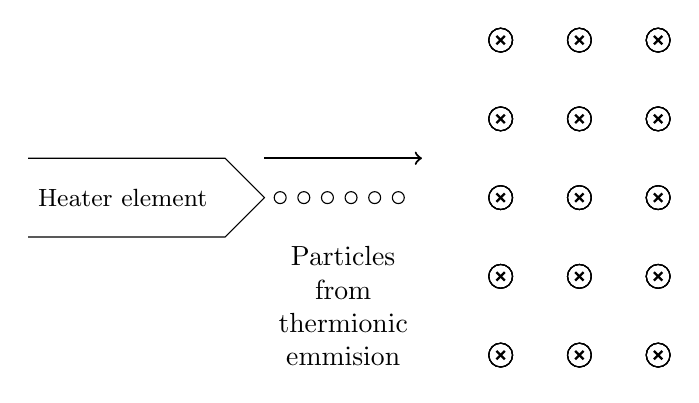
\begin{tikzpicture}
        \begin{scope}[xshift=1cm]
            %% magnetic field into page
            \foreach \x in {0,1,2}
                \foreach \y in {-2,-1,0,1,2}
                    \foreach \z in {45,135,225,315} {
                        \draw[thin]  (\x,\y) circle (1ex);
                        \draw[thick] (\x,\y) -- ++(\z:0.5ex);
                    }
        \end{scope}
        \begin{scope}[xshift=-2cm]
            %% heater element
            \draw (-3,0.5) -- (-0.5,0.5) -- (0,0) -- (-0.5,-0.5) -- (-3,-0.5);
            \node[anchor=west,font=\small] at (-3,0) {Heater element};
            %% particles
            \foreach \x in {2,5,8,11,14,17}
                \draw (\x mm,0) circle (0.5ex);
            \draw[thick,->] (0,0.5) -- (2,0.5);
            \node[anchor=north,text width=6em,text centered] at (1,-0.5) {Particles from thermionic emmision};
        \end{scope}
    \end{tikzpicture}
    \end{center}
    Upon entering the magnetic field,
        the particles will be deflected:
    \begin{choices}
        \wrongchoice{toward the top of the page.}
      \correctchoice{toward the bottom of the page.}
        \wrongchoice{into the page.}
        \wrongchoice{out of the page.}
    \end{choices}
\end{question}
}


%% Section June1995
%%--------------------
\element{nysed}{
\begin{question}{June1995-Q76}
    Which graph best represents the relationship between the degree of deflection of a galvanometer needle and the current passing through its coil?
    \begin{multicols}{2}
    \begin{choices}
        \AMCboxDimensions{down=-2.5em}
        \wrongchoice{
            \begin{tikzpicture}
                \begin{axis}[
                    axis y line=left,
                    axis x line=bottom,
                    axis line style={->},
                    xlabel={current},
                    xtick=\empty,
                    ylabel={deflection},
                    ytick=\empty,
                    xmin=0,xmax=11,
                    ymin=0,ymax=11,
                    width=\columnwidth,
                    very thin,
                ]
                \addplot[line width=1pt,mark=\empty] plot coordinates { (0,5) (5,5) (10,10)};
                \end{axis}
            \end{tikzpicture}
        }
        \wrongchoice{
            \begin{tikzpicture}
                \begin{axis}[
                    axis y line=left,
                    axis x line=bottom,
                    axis line style={->},
                    xlabel={current},
                    xtick=\empty,
                    ylabel={deflection},
                    ytick=\empty,
                    xmin=0,xmax=11,
                    ymin=0,ymax=11,
                    width=\columnwidth,
                    very thin,
                ]
                \addplot[line width=1pt,domain=0:10] {0.1*x*x};
                \end{axis}
            \end{tikzpicture}
        }
        \wrongchoice{
            \begin{tikzpicture}
                \begin{axis}[
                    axis y line=left,
                    axis x line=bottom,
                    axis line style={->},
                    xlabel={current},
                    xtick=\empty,
                    ylabel={deflection},
                    ytick=\empty,
                    xmin=0,xmax=11,
                    ymin=0,ymax=11,
                    width=\columnwidth,
                    very thin,
                ]
                \addplot[line width=1pt,domain=0:10] {10/x};
                \end{axis}
            \end{tikzpicture}
        }
        %% ANS is 4
        \correctchoice{
            \begin{tikzpicture}
                \begin{axis}[
                    axis y line=left,
                    axis x line=bottom,
                    axis line style={->},
                    xlabel={current},
                    xtick=\empty,
                    ylabel={deflection},
                    ytick=\empty,
                    xmin=0,xmax=11,
                    ymin=0,ymax=11,
                    width=\columnwidth,
                    very thin,
                ]
                \addplot[line width=1pt,domain=0:10] {x};
                \end{axis}
            \end{tikzpicture}
        }
    \end{choices}
    \end{multicols}
\end{question}
}

\element{nysed}{
\begin{question}{June1995-Q77}
    The torque on the armature of an operating electric motor may be increased by:
    \begin{choices}
        \wrongchoice{decreasing the current in the armature}
        \wrongchoice{decreasing the magnetic field strength of the field poles}
      \correctchoice{increasing the potential difference applied to the armature}
        \wrongchoice{increasing the distance between the armature and the field poles}
    \end{choices}
\end{question}
}

\element{nysed}{
\begin{question}{June1995-Q78}
    In an operating practical motor,
        the magnetic field produced by the current-carrying coil is strengthened and concentrated by the:
    \begin{choices}
        \wrongchoice{split-ring commutator}
        \wrongchoice{back emf}
        \wrongchoice{field pole}
      \correctchoice{iron core}
    \end{choices}
\end{question}
}

\element{nysed}{
\begin{question}{June1995-Q79}
    The diagram below represents an electron beam entering the region between two oppositely charged parallel plates.
    \begin{center}
    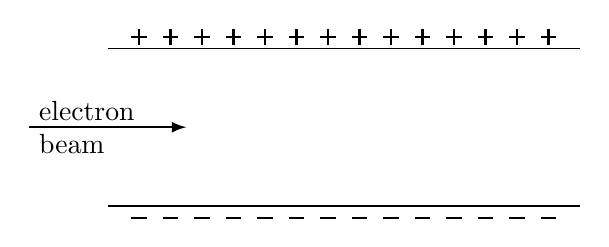
\begin{tikzpicture}
        %% electron beam
        \draw[thick,-latex] (-1,1) -- (1,1) node[pos=0,anchor=west,text width=4em] {electron beam};
        %% bottom plate
        \draw (0,0) -- (6,0);
        \foreach \x in {4,8,...,56}
            \foreach \y in {0,180}
                \draw[thick] (\x mm,-0.15) -- ++(\y:0.1);
        %% top plate
        \draw (0,2) -- (6,2);
        \foreach \x in {4,8,...,56}
            \foreach \y in {0,90,180,270}
                \draw[thick] (\x mm,2.15) -- ++(\y:0.1);
    \end{tikzpicture}
    \end{center}
    In which direction will the beam of electrons be deflected?
    \begin{choices}
        \wrongchoice{out of the page}
        \wrongchoice{into the page}
      \correctchoice{toward the top of the page}
        \wrongchoice{toward the bottom of the page}
    \end{choices}
\end{question}
}

\element{nysed}{
\begin{question}{June1995-Q80}
    A proton having a velocity of \SI{1.5e5}{\meter\per\second} to the right is projected into a magnetic field having a flux density of \SI{3.0}{\tesla} directed out of the page,
        as shown in the diagram below.
    \begin{center}
    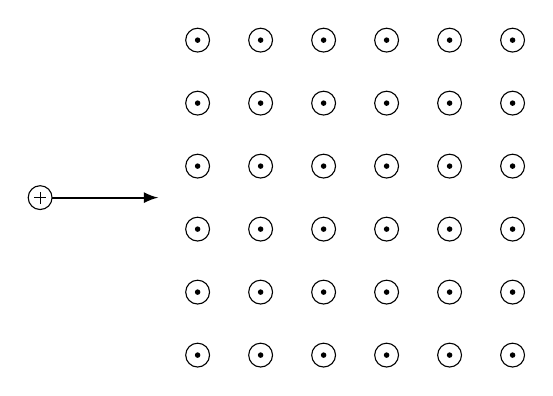
\begin{tikzpicture}
        %% proton
        \draw[thick,-latex] (-2,2) -- (-0.5,2);
        \draw[fill=white] (-2,2) circle (1ex);
        \foreach \z in {0,90,180,270}
            \draw (-2,2) -- ++(\z:0.5ex);
        %% B field
        \foreach \x in {0,8,...,40}
            \foreach \y in {0,8,...,40} {
                \draw (\x mm,\y mm) circle (1ex);
                \fill (\x mm,\y mm) circle (1pt);
            }
    \end{tikzpicture}
    \end{center}
    What is the magnitude of the magnetic force on the proton?
    \begin{multicols}{2}
    \begin{choices}
        \wrongchoice{\SI{4.1e-24}{\newton}}
      \correctchoice{\SI{7.2e-13}{\newton}}
        \wrongchoice{\SI{4.5e6}{\newton}}
        \wrongchoice{\SI{7.2e6}{\newton}}
    \end{choices}
    \end{multicols}
\end{question}
}

\newcommand{\nysedJuneNineteenNinetyFiveQEightyOne}{
\begin{tikzpicture}
    %% B field
    \foreach \x in {-20,-12,...,20}
        \foreach \y in {-20,-12,...,20} {
            \draw (\x mm,\y mm) circle (1ex);
            \fill (\x mm,\y mm) circle (1pt);
        }
    %% options
    \node[anchor=center] (A) at (-4,0) {$A$};
    \draw[thick,-latex] (A.east) -- ++(0:1) node[pos=0.5,anchor=south] {$e^-$};
    \node[anchor=center] (B) at (0,+4) {$B$};
    \draw[thick,-latex] (B.south) -- ++(270:1) node[pos=0.5,anchor=west] {$e^-$};
    \node[anchor=center] (C) at (+4,0) {$C$};
    \draw[thick,-latex] (C.west) -- ++(180:1) node[pos=0.5,anchor=south] {$e^-$};
    \node[anchor=center] (D) at (0,-4) {$D$};
    \draw[thick,-latex] (D.north) -- ++(90:1) node[pos=0.5,anchor=west] {$e^-$};
\end{tikzpicture}
}

\element{nysed}{
\begin{question}{June1995-Q81}
    Four electron beams, $A$, $B$, $C$, and $D$, are projected into a magnetic field directed out of the page.
    \begin{center}
        \nysedJuneNineteenNinetyFiveQEightyOne
    \end{center}
    Which beam of the electrons will initially be deflected toward the top of the page by the magnetic field?
    \begin{multicols}{4}
    \begin{choices}[o]
      \correctchoice{$A$}
        \wrongchoice{$B$}
        \wrongchoice{$C$}
        \wrongchoice{$D$}
    \end{choices}
    \end{multicols}
\end{question}
}

\element{nysed}{
\begin{question}{June1995-Q82}
    Four electron beams, $A$, $B$, $C$, and $D$, are projected into a magnetic field directed out of the page.
    \begin{center}
        \nysedJuneNineteenNinetyFiveQEightyOne
    \end{center}
    If the speed of the electrons in beam $B$ is doubled and the magnetic field strength is halved,
        the magnitude of the deflecting force on the electrons will be:
    \begin{multicols}{2}
    \begin{choices}
      \correctchoice{unchanged}
        \wrongchoice{doubled}
        \wrongchoice{halved}
        \wrongchoice{quadrupled}
    \end{choices}
    \end{multicols}
\end{question}
}

\element{nysed}{
\begin{question}{June1995-Q83}
    The charge to mass ratio of an electron is:
    \begin{multicols}{2}
    \begin{choices}
        \wrongchoice{\SI{9.1e-31}{\coulomb\per\kilo\gram}}
        \wrongchoice{\SI{1.6e-19}{\coulomb\per\kilo\gram}}
        \wrongchoice{\SI{5.7e-12}{\coulomb\per\kilo\gram}}
      \correctchoice{\SI{1.8e11}{\coulomb\per\kilo\gram}}
    \end{choices}
    \end{multicols}
\end{question}
}

\element{nysed}{
\begin{question}{June1995-Q84}
    A potential difference of \SI{10}{\volt} is induced in a wire as it is moved at a constant speed of \SI{5.0}{\meter\per\second} perpendicular to a magnetic field having a flux density of \SI{4.0}{\newton\per\ampere\per\meter}.
    What is the length of the wire in the field?
    \begin{multicols}{2}
    \begin{choices}
      \correctchoice{\SI{0.50}{\meter}}
        \wrongchoice{\SI{2.0}{\meter}}
        \wrongchoice{\SI{8.0}{\meter}}
        \wrongchoice{\SI{200}{\meter}}
    \end{choices}
    \end{multicols}
\end{question}
}

\element{nysed}{
\begin{question}{June1995-Q85}
    The primary coil of an operating transformer has 200 turns and the secondary coil has 40 turns.
    This transformer is being used to:
    \begin{choices}
        \wrongchoice{decrease voltage and decrease current}
      \correctchoice{decrease voltage and increase current}
        \wrongchoice{increase voltage and decrease current}
        \wrongchoice{increase voltage and increase current}
    \end{choices}
\end{question}
}



%% Section June1994
%%--------------------
\element{nysed}{
\begin{question}{June1994-Q34}
    An electromagnet would have the greatest strength if its wires were wrapped around a core made of:
    \begin{multicols}{2}
    \begin{choices}
        \wrongchoice{wood}
      \correctchoice{iron}
        \wrongchoice{aluminum}
        \wrongchoice{copper}
    \end{choices}
    \end{multicols}
\end{question}
}


%% Section June1986
%%--------------------
\newcommand{\nysedJuneNineteenEightySixQNinetyFour}{
\ctikzset{bipoles/length=1.00cm}
\begin{circuitikz}[font=\small]
    %% Circuit
    \draw (0,1) to (0,1.5) to (4,1.5) to [battery,v=$ $] (4,-1.5) to (0,-1.5) to (0,-1);
    %% parallel plates
    \draw[thick] (-1,+1) -- (1,+1);
    \draw[thick] (-1,-1) -- (1,-1);
    %% distance
    \draw[<->] (1.75,0.75) -- (1.75,-0.75) node[pos=0.5,anchor=center,fill=white] {\SI{0.050}{\meter}};
    %% options
    \fill (0,0) circle (1.5pt) node[anchor=west] {$P$};
    \foreach \x/\y in {90/A,0/B,180/D,270/C}
        \fill (\x:0.8) circle (1.5pt) node[anchor=center,shift={({\x+90}:0.75em)}] {$\y$};
    %% electron
    \node[draw,circle] (E) at (-3,0) {$e$};
    \draw[thick,-latex] (E.east) -- ++(0:1.5) node[pos=0.5,anchor=south] {$v$};
\end{circuitikz}
}

\element{nysed}{
\begin{question}{June1986-Q94}
    The diagram below represents two large parallel conducting plates charged to a potential of \SI{10}{\volt}.
    The plates are separated by a distance of \SI{0.050}{\meter}.
    \begin{center}
        \nysedJuneNineteenEightySixQNinetyFour
    \end{center}
    The direction of the electric field at point $P$ is toward point:
    \begin{multicols}{4}
    \begin{choices}[o]
      \correctchoice{$A$}
        \wrongchoice{$B$}
        \wrongchoice{$C$}
        \wrongchoice{$D$}
    \end{choices}
    \end{multicols}
\end{question}
}

\element{nysed}{
\begin{question}{June1986-Q95}
    The diagram below represents two large parallel conducting plates charged to a potential of \SI{10}{\volt}.
    The plates are separated by a distance of \SI{0.050}{\meter}.
    \begin{center}
        \nysedJuneNineteenEightySixQNinetyFour
    \end{center}
    The magnitude of the electric field intensity at point $P$ is:
    \begin{multicols}{2}
    \begin{choices}
        \wrongchoice{\SI{20}{\newton\per\coulomb}}
        \wrongchoice{\SI{2.0}{\newton\per\coulomb}}
        \wrongchoice{\SI{2.0e3}{\newton\per\coulomb}}
      \correctchoice{\SI{2.0e2}{\newton\per\coulomb}}
    \end{choices}
    \end{multicols}
\end{question}
}

\element{nysed}{
\begin{question}{June1986-Q96}
    The diagram below represents two large parallel conducting plates charged to a potential of \SI{10}{\volt}.
    The plates are separated by a distance of \SI{0.050}{\meter}.
    \begin{center}
        \nysedJuneNineteenEightySixQNinetyFour
    \end{center}
    If an electron were projected into the electric field with a velocity $v$,
        it would experience a deflection:
    \begin{choices}
        \wrongchoice{into the page}
        \wrongchoice{out of the page}
        \wrongchoice{toward the top of the page}
      \correctchoice{toward the bottom of the page}
    \end{choices}
\end{question}
}

\element{nysed}{
\begin{question}{June1986-Q97}
    The diagram below represents two large parallel conducting plates charged to a potential of \SI{10}{\volt}.
    The plates are separated by a distance of \SI{0.050}{\meter}.
    \begin{center}
        \nysedJuneNineteenEightySixQNinetyFour
    \end{center}
    Compared to the magnitude of the electric field intensity at point $P$,
        the magnitude of the electric field intensity at point $A$ is:
    \begin{multicols}{3}
    \begin{choices}
        \wrongchoice{less}
        \wrongchoice{greater}
      \correctchoice{the same}
    \end{choices}
    \end{multicols}
\end{question}
}



\endinput


